\documentclass{article}
\usepackage{iclr,times}

% The supplied notation file loads amsmath, amsfonts, and bm.
\input{math.tex}

\usepackage{graphicx}
\usepackage{booktabs}
\usepackage{xcolor}
\usepackage{tikz}
\usetikzlibrary{arrows.meta,positioning}
\usepackage{hyperref}
\usepackage{url}

\newcommand{\method}{\textsc{CoGen}}
\newcommand{\code}[1]{\texttt{#1}}
\newcommand{\ptag}[1]{\texttt{<#1>}}
\newcommand{\tabref}[1]{Table~\ref{#1}}
\newcommand{\appref}[1]{Appendix~\ref{#1}}
\newcommand{\given}{\mathcal{C}}
\newcommand{\modalities}{\mathcal{M}}
\newcommand{\concat}{\mathbin{\|}}
\newcommand{\bigconcat}{\Vert}

\tikzset{
  block/.style={draw, rounded corners=1pt, align=center, minimum height=8mm,
                inner xsep=4pt, font=\small},
  source/.style={block, fill=gray!9},
  frozen/.style={block, fill=blue!9},
  learned/.style={block, fill=orange!13, very thick},
  arrow/.style={-{Latex[length=2mm]}, semithick}
}

\title{Prompt-Routed Multimodal Generation\\with a Shared World--Action Head}

% Authors must remain anonymous for submission.
\author{Anonymous authors\\Paper under double-blind review}

% \iclrfinalcopy  % Uncomment only for the camera-ready version.

\begin{document}
\maketitle

\begin{abstract}
World action models usually predict RGB futures and robot actions, while depth, semantics, and
surface geometry are produced by separate networks or modality-specific heads. We present
\method, a prompt-routed extension of Action Images in which RGB video, metric depth, dense
scene-role segmentation, surface normals, and end-effector actions share one generative output
space. Each signal is represented as an RGB-like video, encoded by the same frozen video VAE,
packed into a common latent sequence, and predicted by the same diffusion-transformer output
projection under one masked flow-matching loss. A task template determines the sequence layout
and is serialized into the language prompt with atomic modality tags; an independent
conditioning plan determines which segments are observed and which are generated. Our principal
training configuration mixes \code{video+action}, \code{video+depth},
\code{video+segmentation}, and \code{video+normal} with probabilities
$0.4/0.2/0.2/0.2$. A preliminary pipeline diagnostic at step 4,500 shows that this single
checkpoint produces all four requested auxiliary streams on the same held-in RLBench episode:
5.4\,cm median action-position error, 0.160 depth AbsRel, 0.373 scene-role macro-mIoU, and
0.904 normal cosine similarity in the joint-generation regime. We distinguish these diagnostic
measurements from a completed benchmark: held-out evaluation, closed-loop evaluation, and
joint depth--action templates remain unreported. We also make explicit that the prompt tag and
the target modality's clean first-frame anchor co-specify the route; prompt-only routing is not
claimed by the present training distribution.
\end{abstract}

\section{Introduction}

World action models (WAMs) learn a policy together with a predictive model of the visual future
\citep{zhu2025unified,zhen2026action}. This joint objective can expose the policy to interaction
dynamics that are absent from action regression alone. Yet the predicted world is usually RGB.
Robotic systems also need geometry, semantics, and surface orientation, and recent methods add
structured supervision through auxiliary branches or experts
\citep{ma2026geosem,yuan2026dreamwam,zhao2026rynnworld}. Such designs are effective, but their
output vocabulary is fixed by the architecture.

A complementary line of work casts visual understanding as image or video generation. Painter
uses images to represent both task demonstrations and outputs \citep{wang2023painter}; Vision
Banana and GenCeption instruction-tune large generators to emit depth, segmentation, normals,
and other visual measurements \citep{gabeur2026image,wang2026video}. SUV applies a shared video
expert to future appearance, semantics, depth, and dynamics in driving, while retaining a
separate action expert \citep{yuan2026suv}. These results suggest that the output representation,
rather than a task-specific decoder, can identify a visual task.

Action Images \citep{zhen2026action} makes this idea directly applicable to manipulation: a
continuous end-effector trajectory is projected into each camera and rendered as a three-channel
Gaussian video. Actions and observations can consequently be denoised in a single video latent
sequence. We extend that interface rather than adding prediction heads. In \method, a sampled
template specifies which modalities occupy the sequence; atomic tags textualize that template;
and a conditioning mask specifies which latent positions are clean. All target positions share
the same VAE, denoiser, final projection, scheduler, and loss.

The distinction between \emph{template} and \emph{conditioning} is important. For example,
\code{video+depth} under full RGB conditioning is depth estimation, whereas the same template
with only initial frames conditioned is a joint RGB--depth world model. Conversely, changing a
tag without changing the segment layout or its target anchor is outside the training support.
We therefore use \emph{prompt-routed} to mean that a prompt-visible task template selects a
trained route, not that text has been causally isolated as the only routing signal.

Our contributions are:
\begin{itemize}
  \item a shared output formulation for RGB, depth, scene-role segmentation, normals, and
  actions, requiring no learned modality-specific head or modality-specific loss;
  \item a factorization of each example into a prompt-serialized modality template and an
  orthogonal conditioning plan, covering joint generation, cross-view generation, inverse
  prediction, single-frame policy learning, and video-only learning;
  \item an auditable arm6 training distribution that preserves prompt--layout--target agreement
  and exact view/time correspondence across all streams; and
  \item a reproducible, deliberately preliminary validation of the arm6 checkpoint, together
  with explicit boundaries around the experiments that have not yet been run.
\end{itemize}

\section{Related Work}

\paragraph{World--action generation.}
Unified World Models couple video and action diffusion while retaining stream-specific noise
levels \citep{zhu2025unified}. Action Images instead renders actions into multiview images and
uses one video-generative process \citep{zhen2026action}; this is our starting checkpoint and
representation. Camera conditioning follows the same Pl\"ucker-ray construction, related to
camera-controlled video generation \citep{sitzmann2021lfn,bai2025recammaster}.

\paragraph{Structured future supervision.}
GeoSem-WAM adds geometry and semantic prediction branches to an RGB future objective
\citep{ma2026geosem}. DreamWAM jointly denoises RGB and motion and uses gated residual branches
for geometry and semantics \citep{yuan2026dreamwam}. RynnWorld-4D co-generates RGB, depth, and
flow with a tri-branch model and obtains actions from an inverse-dynamics head
\citep{zhao2026rynnworld}. SUV is closer to our visual design: a shared video expert emits
several future scene streams without stream-specific visual heads, although action remains a
separate expert \citep{yuan2026suv}. \method differs in placing action and every visual
modality behind the same generative projection.

\paragraph{Understanding through generation.}
Generalist vision models unify heterogeneous targets by representing them as images
\citep{wang2023painter,zhuang2025argus}. Recent image and video generators scale this approach
to broad task mixtures selected by instructions \citep{gabeur2026image,wang2026video}. Our focus
is narrower and embodied: synchronized future RGB, geometric, semantic, and action streams are
packed into the latent sequence of a WAM, and the conditioning pattern is part of the task
definition.

\section{Method}
\label{sec:method}

\subsection{Overview: one ambient space and one head}

Let
\begin{equation}
\modalities=\{\mathrm{video},\mathrm{depth},\mathrm{seg},\mathrm{normal},\mathrm{action}\}.
\label{eq:modalities}
\end{equation}
For each modality $m$, a deterministic codec $c_m$ produces a three-channel clip in
$[-1,1]$. RGB uses the identity codec. Depth, segmentation, and normals use the codecs in
\secref{sec:codecs}; actions are projected and rendered using camera calibration. The same
frozen causal video VAE $E$ maps every clip to
\begin{equation}
  \mathbf{z}_{v,m}=E\!\left(c_m(\mathbf{x}_{v,m})\right)
  \in\mathbb{R}^{C\times T_z\times H_z\times W_z},
\label{eq:sharedvae}
\end{equation}
where $v$ indexes a camera view. Thus modality identity is never represented by choosing a
decoder head. It is represented by the sampled sequence template, its prompt tags, and the
target pixels. The frozen VAE decoder and the inverse codec $c_m^{-1}$ recover the requested
measurement at inference.

\begin{figure}[t]
\centering
\resizebox{0.95\textwidth}{!}{%
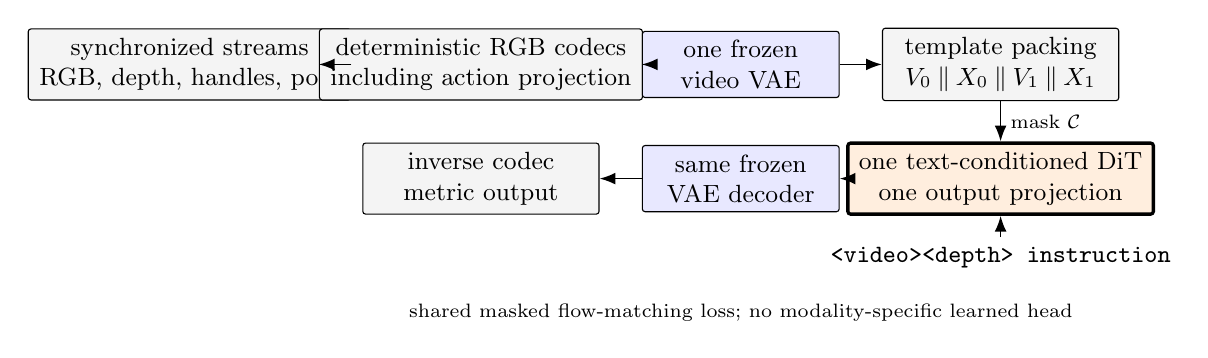
\begin{tikzpicture}
  \node[source, minimum width=30mm] (raw) at (0,0)
    {synchronized streams\\RGB, depth, handles, pose};
  \node[source, minimum width=30mm] (codec) at (3.7,0)
    {deterministic RGB codecs\\including action projection};
  \node[frozen, minimum width=25mm] (vae) at (7.0,0)
    {one frozen\\video VAE};
  \node[source, minimum width=30mm] (pack) at (10.3,0)
    {template packing\\$V_0\concat X_0\concat V_1\concat X_1$};
  \node[learned, minimum width=30mm] (dit) at (10.3,-1.45)
    {one text-conditioned DiT\\one output projection};
  \node[frozen, minimum width=25mm] (dec) at (7.0,-1.45)
    {same frozen\\VAE decoder};
  \node[source, minimum width=30mm] (metric) at (3.7,-1.45)
    {inverse codec\\metric output};
  \draw[arrow] (raw) -- (codec);
  \draw[arrow] (codec) -- (vae);
  \draw[arrow] (vae) -- (pack);
  \draw[arrow] (pack) -- node[right,font=\scriptsize]{mask $\given$} (dit);
  \draw[arrow] (dit) -- (dec);
  \draw[arrow] (dec) -- (metric);
  \node[font=\small\ttfamily] (prompt) at (10.3,-2.45)
    {<video><depth> instruction};
  \draw[arrow] (prompt) -- (dit);
  \node[font=\scriptsize, align=center] at (7.0,-3.15)
    {shared masked flow-matching loss; no modality-specific learned head};
\end{tikzpicture}}
\caption{\method{} converts all outputs to an RGB-like video interface. A task template fixes the
packed layout and is written into the prompt. The only learned predictor is the shared DiT; the
text encoder and video VAE are frozen. $X$ is action, depth, scene-role segmentation, or normal.}
\label{fig:overview}
\end{figure}

\subsection{Prompt-routed task templates}
\label{sec:templates}

A template $\Pi\subseteq\modalities$ specifies the modalities present in an example. Modalities
are sorted in the fixed order
\begin{equation}
\mathrm{video}\prec\mathrm{depth}\prec\mathrm{seg}\prec\mathrm{normal}\prec\mathrm{action},
\label{eq:order}
\end{equation}
and segments are packed view-major and modality-minor:
\begin{equation}
 \mathbf{z}^{\Pi}=\mathop{\bigconcat}_{v=0}^{V-1}
 \mathop{\bigconcat}_{m\in\operatorname{ord}_{\prec}(\Pi)}\mathbf{z}_{v,m},
\label{eq:packing}
\end{equation}
where $\operatorname{ord}_{\prec}$ sorts by \eqref{eq:order} and $\bigconcat$ denotes
concatenation along latent time. With two views,
\code{video+depth} becomes $V_0\concat D_0\concat V_1\concat D_1$. The corresponding prompt is
the bare instruction prefixed by atomic tags, e.g.,
\code{<video><depth> slide the bottom drawer open}. Scene-role segmentation uses the single
atomic tag \ptag{scene-seg}; its palette is fixed globally, so no episode-specific color map is
needed. During training, punctuation is scrubbed by the inherited text path and text is dropped
with probability $0.05$ for classifier-free guidance.

Arm6 uses only the four two-modality templates in \tabref{tab:templates}. These templates all
contain four full-length segments and therefore have the same latent-sequence length. Action
dropout additionally produces a two-segment video-only example. The generic assembler can express
\code{depth+action} and \code{video+depth+action}, but neither template occurs in arm6: depth and
action are trained in separate examples, never jointly in the same packed sequence.

\begin{table}[t]
\caption{The arm6 task menu. $V,D,S,N,A$ denote RGB, depth, scene-role segmentation, normal,
and action. Template choice, prompt prefix, and packed target are constructed together.}
\label{tab:templates}
\centering
\small
\begin{tabular}{lclc}
\toprule
\textbf{Template} & \textbf{Probability} & \textbf{Prompt prefix} & \textbf{Two-view layout} \\
\midrule
\code{video+action}       & $0.40$ & \ptag{video}\ptag{action}    & $V_0\concat A_0\concat V_1\concat A_1$ \\
\code{video+depth}        & $0.20$ & \ptag{video}\ptag{depth}     & $V_0\concat D_0\concat V_1\concat D_1$ \\
\code{video+segmentation} & $0.20$ & \ptag{video}\ptag{scene-seg} & $V_0\concat S_0\concat V_1\concat S_1$ \\
\code{video+normal}       & $0.20$ & \ptag{video}\ptag{normal}    & $V_0\concat N_0\concat V_1\concat N_1$ \\
\bottomrule
\end{tabular}
\end{table}

\subsection{Conditioning plans}
\label{sec:masks}

The template specifies \emph{what} is present; a conditioning plan specifies \emph{what is
given}. For every segment, \code{F} marks the full segment as clean, while \code{I} marks only
its first latent frame as clean. Clean positions form a Boolean set $\given$ and are excluded
from the loss. A \code{1} segment is truncated to one latent frame, which is itself clean. For a
two-view template $V_0\concat X_0\concat V_1\concat X_1$, the implemented plans are:

\begin{table}[t]
\caption{Conditioning plans. \code{I}, \code{F}, and \code{1} denote initial-latent
conditioning, full-segment conditioning, and a clean one-latent segment, respectively. The
single-frame policy plan is action-specific.}
\label{tab:masks}
\centering
\small
\begin{tabular}{llp{7.3cm}}
\toprule
\textbf{Name} & \textbf{Segment states} & \textbf{Interpretation} \\
\midrule
\code{IIII} & I--I--I--I & Jointly generate both streams and both views from their initial latent frames. \\
\code{FIII} & F--I--I--I & Condition on the complete first visual view; generate the remaining segments. \\
\code{FIFI} & F--I--F--I & Condition on both complete primary-visual streams; infer the paired stream. \\
\code{policy} & 1--I--1--I & Keep one clean frame per RGB view and generate full action segments. \\
\code{video-only} & I--I & After action dropout, generate the two RGB views from initial frames. \\
\bottomrule
\end{tabular}
\end{table}

For \code{video+action}, \code{FIFI} is inverse action prediction from observed video. For
\code{video+depth}, it is video-to-depth estimation. Under \code{IIII}, both are generative world
models. The assembler tracks cumulative offsets, so full and one-frame segments can coexist, and
asserts $\given^c\neq\emptyset$; a fully conditioned example would otherwise consume a training
step with zero supervised positions.

\subsection{Shared masked flow matching}

Let $\boldsymbol\epsilon\sim\mathcal{N}(0,I)$ and let $\sigma_t$ be the scheduler noise level.
The full packed sequence is noised as
\begin{equation}
 \mathbf{z}_t=(1-\sigma_t)\mathbf{z}^{\Pi}+\sigma_t\boldsymbol\epsilon,
 \qquad \mathbf{u}=\boldsymbol\epsilon-\mathbf{z}^{\Pi}.
\label{eq:flow}
\end{equation}
After noising, clean positions are restored:
$\widetilde{\mathbf{z}}_{t,i}=\mathbf{z}^{\Pi}_i$ for $i\in\given$ and
$\widetilde{\mathbf{z}}_{t,i}=\mathbf{z}_{t,i}$ otherwise. The text-conditioned DiT
$f_\theta$ receives the packed latents, the timestep, and VAE-encoded Pl\"ucker camera rays.
It is optimized by
\begin{equation}
 \mathcal{L}(\theta)=
 \mathbb{E}_{\Pi,t,\boldsymbol\epsilon,\given}
 \left[
 w_t\,
 \frac{\sum_i \mathbf{1}[i\notin\given]
 \left\|f_\theta(\widetilde{\mathbf{z}}_t,t,\mathbf{c}_{\rm cam},
 \mathbf{c}_{\rm txt})_i-\mathbf{u}_i\right\|_2^2}
 {\sum_i\mathbf{1}[i\notin\given]}
 \right].
\label{eq:loss}
\end{equation}
There is no modality-dependent term or weight in \eqref{eq:loss}. Camera latents for a view are
repeated for every modality segment from that view and injected by the inherited per-block camera
encoders. The text encoder and VAE remain frozen; the denoiser, including its one final output
projection, is fine-tuned.

\subsection{Exact arm6 mixture}
\label{sec:mixture}

The nominal template distribution is given in \tabref{tab:templates}. A
\code{video+action} draw first drops action with probability $0.10$. Conditional on retaining
action, the inherited sampling logic selects \code{policy} with probability $0.10$; otherwise it
selects \code{IIII}/\code{FIII}/\code{FIFI} with probabilities $0.90/0.05/0.05$. Perception
templates use preset M2, directly selecting \code{IIII}/\code{FIII}/\code{FIFI} with
$0.90/0.05/0.05$. The resulting global distribution is
\begin{equation}
 p(\code{IIII},\code{FIII},\code{FIFI},\code{policy},\code{video-only})
 =(0.8316,0.0462,0.0462,0.0360,0.0400).
\label{eq:realizedmix}
\end{equation}
The derivation is in \appref{app:mixture}. Sampling the template and action dropout in the dataset
ensures that the tags, packed layout, and available targets agree before the forward pass.

\subsection{Modality codecs}
\label{sec:codecs}

\paragraph{Action images.}
An action is $\mathbf{a}_t=(\mathbf{p}_t,R_t,g_t)$: 3D position, orientation, and gripper
openness. For view $v$ with projection $\pi_v$, the renderer projects the gripper center and two
tool-frame axis tips,
\begin{equation}
 \mathbf{q}_{r}=\pi_v(\mathbf{p}_t),\qquad
 \mathbf{q}_{g}=\pi_v(\mathbf{p}_t+\ell R_t\mathbf{e}_x),\qquad
 \mathbf{q}_{b}=\pi_v(\mathbf{p}_t-\ell R_t\mathbf{e}_z),
 \quad \ell=0.1\,\mathrm{m},
\label{eq:actionpoints}
\end{equation}
and draws one Gaussian per channel,
\begin{equation}
 A_{t,c}^{v}(\mathbf{x})=
 \exp\!\left(-\frac{\|\mathbf{x}-\mathbf{q}_c\|_2^2}{2s^2}\right),
 \qquad s=0.05\min(H,W).
\label{eq:actionrender}
\end{equation}
When the gripper is open, weak pixels in the blue channel are floored at $0.25$. At decoding,
channel peaks from two views define rays whose multiview agreement recovers the 3D pose and
orientation \citep{zhen2026action}. Rendering occurs inside the forward pass, so the same 3D
trajectory is reprojected through the exact cameras selected for the RGB sample.

\paragraph{Metric depth.}
Depth $d$ is compressed with
\begin{equation}
 y=1-\left(1-\frac{d}{\lambda c}\right)^{\lambda+1},
 \qquad \lambda=-3,\quad c=10/3,
\label{eq:barron}
\end{equation}
then linearly embedded along the seven-edge RGB-cube path black--red--yellow--green--cyan--blue--
magenta--white \citep{gabeur2026image}. Decoding projects RGB onto the nearest path segment and
inverts \eqref{eq:barron}. Values outside the strict $0.05$--$10$\,m engineering range use an
off-path sentinel and decode as invalid rather than as plausible depth.

\paragraph{Surface normals.}
Normals are derived from synchronized metric depth and camera intrinsics, without additional
annotation. For pixel coordinates $(u,v)$,
\begin{equation}
 \mathbf{n}\propto
 \left(-\frac{f_x}{z}\frac{\partial z}{\partial u},
       -\frac{f_y}{z}\frac{\partial z}{\partial v},1\right)^{\!\top},
 \qquad c_{\rm normal}(\mathbf{n})=\frac{\mathbf{n}+1}{2}.
\label{eq:normal}
\end{equation}
Focal lengths are scaled when depth is resized. The decoder maps RGB back to $[-1,1]^3$ and
renormalizes each vector.

\paragraph{Dense scene roles.}
Raw CoppeliaSim handle maps are converted by a per-episode handle-to-role lookup and a fixed
palette. The semantic roles are background, target, goal, robot arm, gripper, distractor, tool,
and fixture; \code{unknown} is a reserved debugging label that is required to be absent from
training targets. Instruction resolution promotes only manipulable distractors to target, while
preserving goal and tool identities. Compared with instruction-referring targets, the scene-role
maps expose substantially denser supervision: across the 16 tasks, the cross-task median target
coverage is $0.97\%$ for referring masks and $12.19\%$ for non-background scene roles, a
$12.6\times$ increase. The tag is the atomic \ptag{scene-seg} because the role palette is global.

\section{Experimental Protocol and Current Evidence}
\label{sec:experiments}

\subsection{Data and training configuration}

We use a self-generated RLBench dataset \citep{james2020rlbench} with Colosseum-style visual and
camera randomization \citep{pumacay2024colosseum}. It contains 1,028 episodes from 16 tasks, four
calibrated views, and synchronized RGB, metric depth, object-handle masks, camera parameters, and
7-DoF end-effector states. Training uses the 788 variation-0 episodes. Variations 1 and 2 contain
130 and 110 episodes, respectively, and form a 240-episode held-out set that has not yet been
evaluated. Each example samples two of the four views and 41 frames at native stride 3, spanning
121 simulator steps (6.0\,s at approximately 6.7\,Hz).

We warm-start from the released Action Images checkpoint and fine-tune Wan2.2-TI2V-5B
\citep{wan2025}. The actual arm6 run uses $512\times512$ inputs, two GPUs, per-device batch size
1, gradient accumulation 2 (effective global batch 4), bf16, full-denoiser fine-tuning, gradient
checkpointing, and ZeRO-2 with CPU-offloaded optimizer state. Adam uses learning rate
$5\times10^{-7}$, 1,000 warm-up steps, then a constant schedule. The seed is 42. The text
encoder and VAE are frozen. The current checkpoint is step 4,500 of a planned 10,000; the run is
therefore not treated as converged.

\subsection{Metrics and evaluation scope}

Depth is decoded to meters and scored by AbsRel. Scene-role segmentation uses macro-IoU over
roles present in the ground truth. Normals use mean cosine similarity. Actions are decoded from
the two-view heatmaps and scored by median 3D position error and geodesic rotation error.
\code{IIII} is the principal generative regime; \code{FIII}, \code{FIFI}, and \code{policy}
diagnose other conditioning plans that occur during training.

All results in \tabref{tab:diagnostic} use the same arm6 step-4,500 weights, the same held-in
episode (\code{open\_drawer/variation0/episode0}), resolution, temporal stride, and random seed.
They validate routing, decoding, and metric plumbing; $n=1$ does not support a generalization
claim or a comparison to prior methods.

\begin{table}[t]
\caption{Preliminary arm6 diagnostic from one held-in episode at step 4,500. The same checkpoint
is invoked with a different template prefix for each row. Best values across conditioning modes
are not emphasized because the modes expose different amounts of information.}
\label{tab:diagnostic}
\centering
\small
\begin{tabular}{llccc}
\toprule
\textbf{Prompt route} & \textbf{Metric} & \code{IIII} & \code{FIII} & \code{FIFI} \\
\midrule
\ptag{video}\ptag{action} & position med. (cm) $\downarrow$ & 5.40 & 4.50 & 1.85 \\
                           & rotation med. ($^\circ$) $\downarrow$ & 20.89 & 19.81 & 18.73 \\
\ptag{video}\ptag{depth} & AbsRel $\downarrow$ & 0.160 & 0.069 & 1.335 \\
\ptag{video}\ptag{scene-seg} & macro-mIoU $\uparrow$ & 0.373 & 0.355 & 0.494 \\
\ptag{video}\ptag{normal} & mean cosine $\uparrow$ & 0.904 & 0.937 & 0.952 \\
\bottomrule
\end{tabular}
\end{table}

The diagnostic establishes a limited but necessary fact: all four routes produce outputs that
survive their inverse codecs and yield non-degenerate task metrics from one shared checkpoint.
The information ordering is reflected in the action row: observing two full RGB clips
(\code{FIFI}) is easier than jointly imagining RGB and action (\code{IIII}). The depth
\code{FIFI} result moves in the opposite direction and is unstable on this episode. This mode
receives only $4.62\%$ of all arm6 samples, shared across perception and action templates; the
single example cannot distinguish under-training from episode-specific failure. Under
\code{policy}, which receives only single RGB frames, action position and rotation errors are
14.79\,cm and $26.93^\circ$ on the same episode.

As a small cross-episode check, \code{IIII} depth AbsRel at step 4,500 is 0.160, 0.065, 0.116,
and 0.059 on one held-in episode each from \code{open\_drawer}, \code{push\_buttons},
\code{stack\_wine}, and \code{turn\_tap} (mean 0.100). We keep this observation in prose because
four training-variation episodes are still a pipeline check, not the planned held-out sweep.

\section{Discussion and Limitations}
\label{sec:limitations}

\paragraph{The routing signal is not isolated.}
Every predicted segment receives a clean first latent frame. For a depth target, for example,
that anchor is already a depth-encoded image. The modality tag, sequence position, and target
anchor therefore agree throughout training. The present results establish switching through the
complete template interface, not switching caused by text alone. We deliberately do not report
\code{f0f0}: it removes the target anchors, is absent from training, and would be an
out-of-distribution test rather than a clean prompt ablation. A valid causal test requires adding
tag-only examples to the training distribution.

\paragraph{No joint structured-action target.}
Arm6 trains \code{video+action} and each \code{video+structured-modality} template separately.
It has not trained \code{depth+action} or \code{video+depth+action}. Consequently, the current
checkpoint does not establish that depth and action can be generated jointly or that separately
sampled routes are mutually consistent. A three-modality template is supported by the assembler
but increases sequence length from four to six segments.

\paragraph{Incomplete evaluation.}
The principal run has reached 4,500 of 10,000 planned steps and uses one seed. The 240 held-out
variation episodes, closed-loop rollouts, matched action-only and per-modality controls, and
checkpoint selection study have not been completed. We therefore avoid claims about task
generalization, policy success, interference, or superiority to specialized heads. Results from
other exploratory arms are not used as evidence for arm6.

\paragraph{Simulation supervision and consistency.}
Depth, handles, and calibration are simulator ground truth. Real-data extension will require
sensor depth or pseudo-labels whose metric scale and temporal consistency are verified. Moreover,
a shared head and shared latent space do not guarantee physical agreement between outputs from
separate stochastic generations; explicit joint templates or cross-modal consistency objectives
would be needed to test that property.

\section{Conclusion}

\method{} treats modality as part of a WAM's generative interface rather than as an architectural
branch. Deterministic RGB-like codecs place video, actions, depth, scene roles, and normals in the
same frozen-VAE space; a prompt-visible task template specifies their packed layout; a separate
mask specifies what is observed; and one DiT projection is trained with one masked flow-matching
objective. The arm6 diagnostic confirms that this pipeline can route four auxiliary outputs
through one checkpoint. The next empirical requirement is clear: finish arm6, evaluate the
held-out variations and closed loop, and compare against matched controls without introducing
untrained prompt-only or depth--action conditions.

\subsubsection*{Reproducibility Statement}
The launcher records the template mix, conditioning preset, segmentation protocol, dataset,
resolution, temporal stride, seed, and initialization in the output path or run configuration.
The dataset records the sampled frame indices, view indices, and view directories and uses that
provenance for every modality. Startup checks validate requested modality availability,
segmentation coverage, absence of the reserved unknown role, and non-empty prediction masks.
Exact commands and artifact paths for the reported diagnostics are listed in
\code{paper/README.md}.

\bibliography{reference}
\bibliographystyle{iclr}

\appendix

\section{Codec and data-integrity details}
\label{app:codecs}

\paragraph{Depth inversion.}
For an RGB value $\boldsymbol\gamma$, decoding searches the seven RGB-cube edges with endpoints
$(\mathbf{v}_k,\mathbf{v}_{k+1})$:
\begin{equation}
 (k^\star,\alpha^\star)=
 \arg\min_{\substack{k\in\{0,\ldots,6\}\\\alpha\in[0,1]}}
 \left\|\boldsymbol\gamma-\big[(1-\alpha)\mathbf{v}_k+
 \alpha\mathbf{v}_{k+1}\big]\right\|_2^2,
 \qquad \hat y=\frac{k^\star+\alpha^\star}{7}.
\label{eq:depthdecode}
\end{equation}
The inverse is
$\hat d=\lambda c\,[1-(1-\hat y)^{1/(\lambda+1)}]$.
Pixels whose squared distance to the path exceeds 0.15, or whose recovered depth is outside the
valid interval, decode to NaN. Depth is resized with nearest-neighbor interpolation before
encoding so that no metric values are synthesized by the resize operation.

\paragraph{Scene-role palette.}
The fixed sRGB colors are background $(0,0,0)$, target $(230,25,75)$, goal $(60,180,75)$,
robot arm $(0,130,200)$, gripper $(70,240,240)$, distractor $(255,225,25)$, tool
$(240,50,230)$, fixture $(145,30,180)$, and reserved unknown $(245,130,48)$. Decoding is
nearest-palette classification restricted to roles that can legally appear in the episode. It
does not prune small connected components because several valid target objects occupy only a few
pixels. The CoppeliaSim no-object value, truncated to \code{0xFFFF} in the stored mask, maps to
background rather than unknown.

\paragraph{Frozen-VAE checks.}
Stored admission checks provide two useful upper-bound measurements. On 12 episodes, normal clips
round-tripped through the frozen VAE at mean cosine 0.9906 (mean angular error
$7.88^\circ$). On 48 episodes evaluated at $256^2$, scene-role targets had median IoU 0.965 after
the VAE round-trip; the RGB control PSNR was 29.59\,dB. These checks validate representational
survival, not learned prediction quality. We do not report an unstored numeric VAE gate for depth
or action.

\paragraph{Alignment invariants.}
Every perception stream is loaded with the exact frame indices and view directories chosen by the
RGB loader. Each camera's Pl\"ucker embedding is then duplicated for all modality segments from
that camera. Requested templates unsupported by a dataset fail at startup rather than being
silently shortened. For scene roles, all 788 training episodes have target metadata; startup
probes find no reserved-unknown ground-truth pixels.

\section{Realized arm6 probabilities}
\label{app:mixture}

\begin{table}[h]
\caption{Probability decomposition for a nominal \code{video+action} draw. These probabilities
sum to one within that template before multiplying by its arm6 weight of 0.4.}
\label{tab:actionmix}
\centering
\small
\begin{tabular}{lcc}
\toprule
\textbf{Outcome} & \textbf{Composition} & \textbf{Within-template probability} \\
\midrule
video-only & $0.10$ & $0.1000$ \\
\code{policy} & $0.90\times0.10$ & $0.0900$ \\
\code{IIII} & $0.90\times0.90\times0.90$ & $0.7290$ \\
\code{FIII} & $0.90\times0.90\times0.05$ & $0.0405$ \\
\code{FIFI} & $0.90\times0.90\times0.05$ & $0.0405$ \\
\bottomrule
\end{tabular}
\end{table}

Perception templates jointly carry probability 0.6 and use M2, contributing $0.54$ to
\code{IIII} and $0.03$ each to \code{FIII} and \code{FIFI}. The action template contributes
$0.2916$, $0.0162$, $0.0162$, $0.036$, and $0.04$ to \code{IIII}, \code{FIII}, \code{FIFI},
\code{policy}, and video-only, respectively. Summing the two sources gives
\eqref{eq:realizedmix}.

\section{Condition-mask construction}

For a full-length latent segment with temporal length $T_z$, an \code{I} state marks the first
latent slice as clean and leaves $T_z-1$ slices as prediction targets. An \code{F} state marks all
$T_z$ slices clean. A \code{1} state first truncates the segment to one slice, then marks that
slice clean. Offsets are accumulated from the realized segment lengths rather than computed as
multiples of $T_z$; this is required for the \code{policy} layout
$[V_0^{1}\concat A_0\concat V_1^{1}\concat A_1]$. The loss mask uses
\code{True=clean/given}; \eqref{eq:loss} explicitly complements it.

\section{Evaluation status and number provenance}
\label{app:provenance}

\begin{table}[h]
\caption{Status of the empirical cells discussed in the paper. ``Done'' here means that a stored
artifact exists, not that the scope is sufficient for a final benchmark.}
\label{tab:status}
\centering
\small
\begin{tabular}{lll}
\toprule
\textbf{Cell} & \textbf{Status} & \textbf{Scope} \\
\midrule
arm6 step-4,500 route grid & Done & one held-in episode, all trained routes \\
arm6 depth spot check & Done & four held-in episodes \\
normal frozen-VAE round-trip & Done & 12 episodes \\
scene-role frozen-VAE round-trip & Done & 48 episodes at $256^2$ \\
arm6 held-out variations 1--2 & Not done & planned 240 episodes \\
arm6 closed-loop policy & Not done & no success-rate claim \\
arm6 matched controls & Not done & no comparative claim \\
\code{depth+action} / \code{video+depth+action} & Not trained & excluded from results \\
prompt-only target without anchor & Not trained & \code{f0f0} excluded \\
\bottomrule
\end{tabular}
\end{table}

The route-grid numbers come from
\code{reports/modality\_mode\_grid/arm6\_4500/metrics.json}. The additional depth measurements
come from the three sibling \code{arm6\_4500\_ep\_*} directories. Frozen-VAE measurements come
from \code{reports/vae\_roundtrip\_normal.txt} and
\code{reports/vae\_roundtrip\_seg.txt}. Dataset counts and segmentation-density statistics are
recomputed from the active \code{rlbench\_selfgen\_512\_aug} tree and
\code{reports/seg\_pixel\_stats.csv}, respectively.

\section{Reproduction command}

The principal run is launched from the repository root with
\begin{verbatim}
GPUS=1,2 bash scripts/train_arm.sh arm6
\end{verbatim}
which resolves to
\begin{verbatim}
video+action@0.4,video+depth@0.2,
video+segmentation@0.2,video+normal@0.2
\end{verbatim}
with \code{SEG\_MODE=scene\_roles} and \code{PERCEPTION\_MASK\_MIX=M2}. The current run's logged
configuration records gradient accumulation 2; this runtime value, rather than the launcher's
default value, is the one reported in the paper.

\end{document}
